\scanpage{24}
\figure{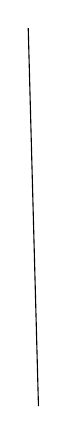
\begin{tikzpicture}\draw (0,0) -- (0.13,-4.8);\end{tikzpicture}}

a) Le foncteur $\omega_N$ (de la catégorie des $k$-modules vers celle des $S$-modules gradués) est pleinement fidèle.

b) \inserted{$\forall M$,} l'application
\diagram{\begin{tikzcd}
M \arrow[r,"\varphi"] & \displaystyle\prod_{i\geq0}\omega_N(M)_i=\prod_{i\geq N}M.T^{(i)}
\end{tikzcd}}
donnée par
\[
\varphi(x)=(x.T^{(i)})_{i\geq N}
\]
induit une bijection de $M$ avec le sous-ens. de $\prod_{i\geq N}\deleted{\unsure{M}}\omega_N(M)_i$ formé des systèmes $(x_i)_{i\geq N}$ satisfaisant la condition
\[
(*)\qquad T^{(j)}x_i=c_{ij}x_{i+j}\qquad\forall i\geq N,\ j\geq1.
\]

\uline{Dém}

b) $x_i=xT^{(i)}$, on a $T^{(j)}x_i=xT^{(i)}T^{(j)}=c_{ij}xT^{(i+j)}=c_{ij}x_{i+j}$, donc $\varphi(x)$ se trouve dans le sous-gr. indiqué.

L'injectivité de $\varphi$ est claire. Bijectivité? Posons $x_i=\unsure{\xi_i|\zeta_i}T^{(i)}$, $\unsure{\xi_i|\zeta_i}\in M$. La condition $(*)$ s'écrit
\[
\begin{array}{ccc}
\xi_iT^{(i)}T^{(j)}&=&c_{ij}\xi_{i+j}T^{(i+j)}\\
\text{''}&&\\
c_{ij}\xi_iT^{(i+j)}&&
\end{array}
\]
i.e.
\[
c_{ij}(\xi_{i+j}-\xi_i)=0\qquad\text{pour }i\geq N,\ j\geq1,
\]
et il résulte du th. que les $\xi_i$ sont tous \uline{égaux} à un $=\xi\in M$, cqfd.

a) Soient $M,M'$ sur $k$. Alors $\operatorname{Hom}(\omega_N(M),\omega_N(M'))$ s'identifie à l'ens des systèmes de $k$-lin $(i\geq N)$
\diagram{\begin{tikzcd}
u_i:\ M \arrow[r,dash] \arrow[d,phantom,"\unsure{\wr|\simeq}" description] & M' \arrow[d,phantom,"\unsure{\wr|\simeq}" description]\\
M.T^{(i)} \arrow[d,phantom,"\text{''}" description] & M'.T^{(i)} \arrow[d,phantom,"\text{''}" description]\\
\omega_N(M)_i & \omega_N(M')_i
\end{tikzcd}}
\mspage{23}
